% !TEX root =  ../pers_schedules.tex

\section{Personalized schedules for patients in PRIAS}
\label{sec : pers_schedule_PRIAS}
To demonstrate how the personalized schedules work, we apply them to the patients enrolled in PRIAS. To this end, we divide the PRIAS dataset into a training dataset with 5264 patients and a demonstration dataset with 3 patients who never experienced GR. We fit a joint model to the training dataset and then use it to create personalized schedules for patients in demonstration dataset. We fit the joint model using the R package JMbayes \citep{rizopoulosJMbayes}, which uses the Bayesian methodology to estimate the model parameters.

\subsection{Fitting the joint model to PRIAS dataset}
\label{subsec : jm_fit_prias}
The training dataset contains age at the time of induction in PRIAS, PSA levels and the time interval in which GR is detected, for 5264 prostate cancer patients. PSA was measured at every 3 months for first 2 years and every 6 months thereafter. To detect GR, biopsies were conducted as per the PRIAS schedule (Section \ref{sec : introduction}). For the longitudinal analysis of PSA we use $\log_2 \mbox{PSA}$ measurements instead of the raw data. This because the PSA scores take very large values around the time of disease progression, indicating that the underlying distribution for PSA is right skewed. The longitudinal sub-model of the joint model we fit is given by:
\begin{equation}
\label{eq : long_model_prias}
\begin{aligned}
\log_2 \mbox{PSA}(t) &= \beta_0 + \beta_1 (Age-70) + \beta_2 (Age-70)^2 + \sum_{k=1}^4 \beta_{k+2} B_k(t,\mathcal{K})\\ 
&+  b_{i0} + b_{i1} B_7(t, 0.1) + b_{i2} B_8(t, 0.1) +
\varepsilon_i(t).
\end{aligned}
\end{equation}
where $B_k(t, \mathcal{K})$ denotes the $k$-th basis function of a B-spline with 3 internal knots at $\mathcal{K} =\{0.1, 0.5, 4\}$ years, and boundary knots at 0 and 7 years. The spline for the random effects consists of 1 internal knot at 0.1 years and boundary knots at 0 and 7 years. The choice of knots was based on exploratory analysis as well as on model selection criteria AIC and BIC. Age of patients was median centered to avoid numerical instabilities during parameter estimation. For the relative risk sub-model the hazard function we fit is given by:
\begin{equation}
\label{eq : hazard_prias}
h_i(t) = h_0(t) \exp\big[\gamma_1 (Age-70)  + \gamma_2 (Age-70)^2 + \alpha_1 m_i(t) + \alpha_2 m'_i(t)\big].
\end{equation}
where $\alpha_1$ and $\alpha_2$ are measures of strength of the association between hazard of GR and $\log_2 \mbox{PSA}$ value $m_i(t)$ and $\log_2 \mbox{PSA}$ velocity $m'_i(t)$, respectively. Since the PRIAS schedule depends only on the observed PSA values (via PSA-DT), the interval censoring observed in PRIAS is independent and non informative of the underlying health of the patient.

From the joint model fitted to the PRIAS dataset we found that only $\log_2 \mbox{PSA}$ velocity was strongly associated with hazard of GR. For any patient, a unit increase in $\log_2 \mbox{PSA}$ velocity led to an 11 times increase in the hazard of GR. The parameter estimates for the fitted joint model are presented in detail in Web Appendix C of the supplementary material. 

\subsection{Demonstration of personalized schedules}
\label{subsec : demo_prias_pers_schedule}
Using the demonstration dataset, we next present the functioning of personalized schedules based on expected time of GR and dynamic risk of GR. The first patient of interest is patient 3174. Since no repeat biopsies were conducted for this patient in the time period we considered, $g(T^*_j)$ depends only on the PSA levels. The evolution of PSA, repeat biopsy history and proposed times of biopsies are shown in Figure \ref{fig : prias_demo_pid_3174}. It can be seen that the schedule of biopsy based on expected time of GR adjusts the times of biopsy according to the rise in hazard (which increases due steep rise in $\log_2 \mbox{PSA}$ velocity) after year 2. More specifically, at year 2 the proposed biopsy time is 12.5 years whereas at year 4 it decreases to 5.3 years. For schedules based on dynamic risk of GR, the optimal $1 - \kappa$ value was found to be between 0 and 0.1 at all time points, because of the sharp rise in PSA values. This value of $\kappa$ corresponds to a time very close to the time of latest biopsy (time 0). Hence the biopsies are scheduled much earlier than those based on expected time of GR.

%On average, a biopsy scheduled using expected time of GR at year 2 should have a larger offset $O^S_j$ compared to the same at year 4. This because $\mbox{var}_g(T^*_j)$ is considerably lower at year 4 as shown in Figure \ref{fig : variance_pred_dist_3174_911}. As expected the variance also strongly depends on $\log_2 \mbox{PSA}$ velocity. 

\begin{figure}
\centerline{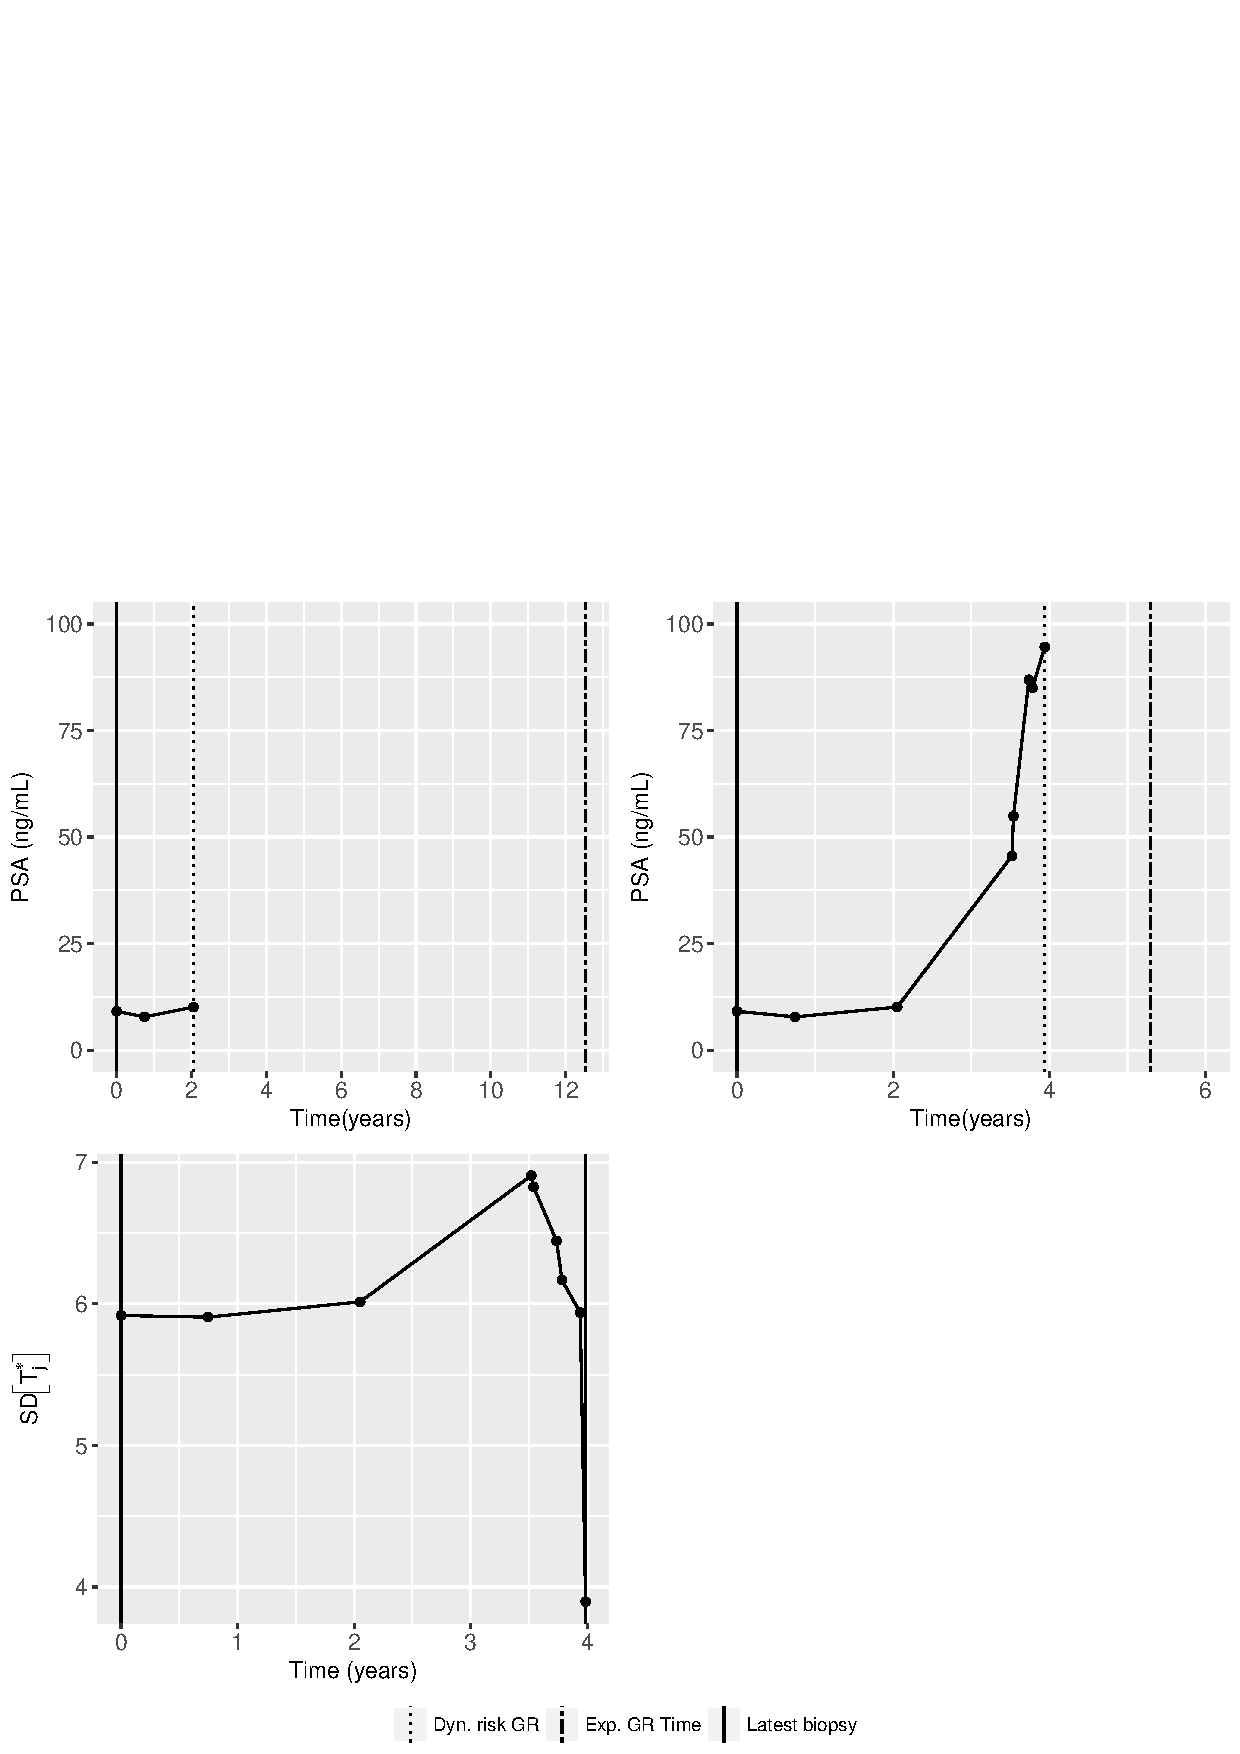
\includegraphics[width=\columnwidth]{images/prias_demo/case_3174.png}}
\caption{PSA and repeat biopsy history, and corresponding personalized schedules for patient 3174.}
\label{fig : prias_demo_pid_3174}
\end{figure}

%\begin{figure}
%\centerline{\includegraphics[width=\columnwidth]{images/prias_demo/variance_3174_911.png}}
%\caption{Standard deviation $\mbox{SD}[T^*_j] = \sqrt{\mbox{var}_g(T^*_j)}$ over time for patient 3174 and 911. Solid vertical lines indicate biopsies.}
%\label{fig : variance_pred_dist_3174_911}
%\end{figure}

The second patient of interest is patient 911, for whom the evolution of PSA, time of last biopsy and proposed biopsy times are shown in Figure \ref{fig : prias_demo_pid_911}. We can see the combined effect of decreasing PSA levels and a negative repeat biopsy on personalized schedules, between year 3 and year 4.5 for this patient. In accordance with the observed history of the patient, the proposed time of biopsy based on expected time of GR increases from 16.6 years to 18.7 years in this period. For dynamic risk of GR it increases from 3.2 years to 15 years, despite the optimal $\kappa$ being equal to 0.98 for the entire period. 

%We can also see that after each repeat biopsy $\mbox{var}_g(T^*_j)$ decreases sharply (Figure \ref{fig : variance_pred_dist_3174_911}), thus in turn reducing the offset as well.

\begin{figure}
\centerline{
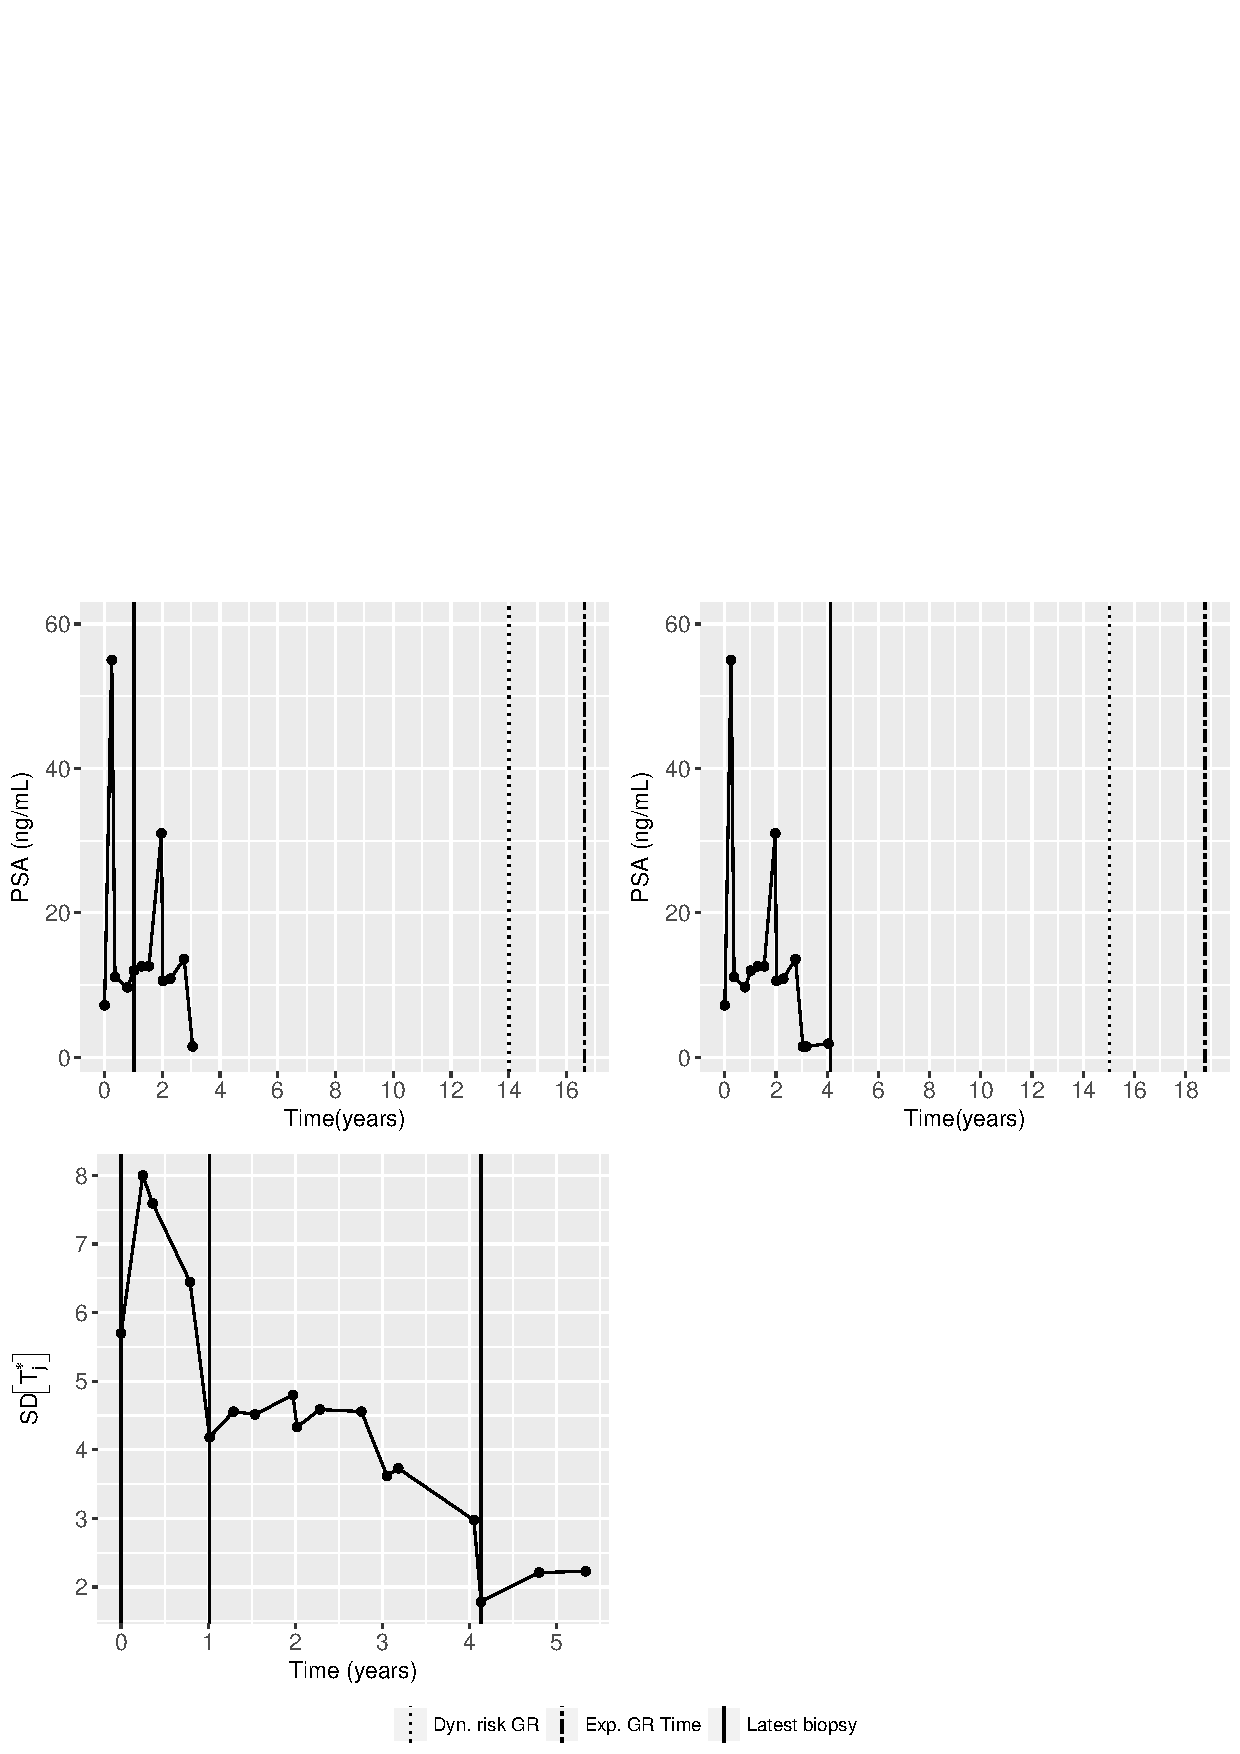
\includegraphics[width=\columnwidth]{images/prias_demo/case_911.png}
}
\caption{PSA and repeat biopsy history, and corresponding personalized schedules for patient 911.}
\label{fig : prias_demo_pid_911}
\end{figure}

Patient 2340 presents a case where information from PSA levels and repeat biopsies is conflicting. In Figure \ref{fig : prias_demo_pid_2340} we can see that the PSA for this patient becomes twice between year 2 and year 3.2. If only information from PSA is considered, then we can see that proposed time of biopsy based on expected time of GR is preponed from 12.5 to 11.5 years during this period. However, if we also take into account the negative result from the repeat biopsy at year 2.5, then the proposed time of biopsy is postponed from 12.5 years to 15 years. Thus more weight is given to a recent negative biopsy result than PSA, which is in accordance with the clinical practice. The proposed time of biopsy based on dynamic risk of GR is also postponed in light of the negative biopsy result.

\begin{figure}
\centerline{\includegraphics[width=\columnwidth]{images/prias_demo/case_2340.png}}
\caption{PSA and repeat biopsy history, and corresponding personalized schedules for patient 2340.}
\label{fig : prias_demo_pid_2340}
\end{figure}

The impact of evolution of PSA levels and repeat biopsy history on the variance of $g(T^*_j)$ is presented in Web Appendix ??? of the supplementary material.